% --------------------------------------------------------------
% This is all preamble stuff that you don't have to worry about.
% Head down to where it says "Start here"
% --------------------------------------------------------------
\documentclass[12pt]{article}

\usepackage[margin=1in]{geometry} 
\usepackage{amsmath,amsthm,amssymb}
\usepackage[UTF8]{ctex}  % 用于中文
\usepackage{graphicx}  % 添加这行来加载插图功能
\usepackage{listings}  % 插入代码功能
\usepackage{xcolor}  % 用于颜色设置
\lstset{
    basicstyle=\ttfamily,         % 设置代码字体为等宽字体
    keywordstyle=\color{blue},    % 关键字颜色
    stringstyle=\color{red},      % 字符串颜色
    commentstyle=\color{green},   % 注释颜色
    breaklines=true,              % 自动换行
    frame=single,                 % 使用单线框包围代码
    showspaces=false,             % 不显示空格
    showstringspaces=false,       % 字符串中的空格不显示
    showtabs=false,               % 不显示制表符
    tabsize=4,                    % 设置 Tab 为 4 个空格
    breaklines=true,              % 允许长行自动换行
}
\linespread{1.0}  % 设置1倍行间距
\usepackage{geometry}
% \usepackage{datetime}
\geometry{
    left=2cm,
    right=2cm,
    top=3cm,
    bottom=3cm,
}
\usepackage{titling}
\usepackage[pagebackref]{hyperref} % 引用
\usepackage{cleveref}
\crefname{figure}{Fig}{Figs}

\begin{document}
\renewcommand{\labelitemii}{$\circ$} % 第二层级符号为圆圈

% --------------------------------------------------------------
%                         Start here
% --------------------------------------------------------------

\setlength{\droptitle}{-3cm}
\title{基础实验:实验报告(模板)}
\author{姓名:xxx \and 学号:xxx}
\date{2024年xx月xx日}
\maketitle


\section{问题分析}

这个问题你是怎么抽象成数据结构问题的?编程时需要完成哪些内容?


\section{数据结构设计与实现}

\subsection{ADT设计}

\begin{itemize}
    \item 数据对象:
    \item 数据关系:
    \item 基本操作:
\end{itemize}

\subsection{ADT 的物理实现}

需要列出构建数据对象的代码片段。

\begin{itemize}
    \item C语言代码展示举例,C++语言只需修改参数为\texttt{[language=C++]}
\end{itemize}
\begin{lstlisting}[language=C]
#include <stdio.h>

int main() {
    for (int i = 0; i < 10; i++) {
        printf("Hello, World!\n");
    }
    return 0;
}
\end{lstlisting}




\section{算法设计与实现}

\subsection{算法设计}

简要说明解决这个问题所需要的算法思想与步骤,并分析该算法的时间/空间复杂度分析。

\begin{itemize}
    \item 时间复杂度分析:
    \item 空间复杂度分析:
\end{itemize}

\subsection{算法实现}

列出完成具体算法所需的关键代码片段,并简单介绍。


\section{实验环境}
\begin{itemize}
    \item 硬件环境:CPU 型号、内存
    \item 软件环境:操作系统、编程语言、IDE及版本等
\end{itemize}

\section{实验结果与分析}

某个操作后,展示并分析对应实验结果。

展示图片\cref{fig:show}如下。

\begin{figure}[htb!]
    % [htb!]:
    % h: 尽量将图片放在当前位置 (here)
    % t: 如果当前位置不合适,将图片放在页面顶部 (top)
    % b: 如果页面顶部也不合适,则放在页面底部 (bottom)
    % !: 强制 LaTeX 忽略浮动体的一些限制,尽量按指定位置放置
    \centering
    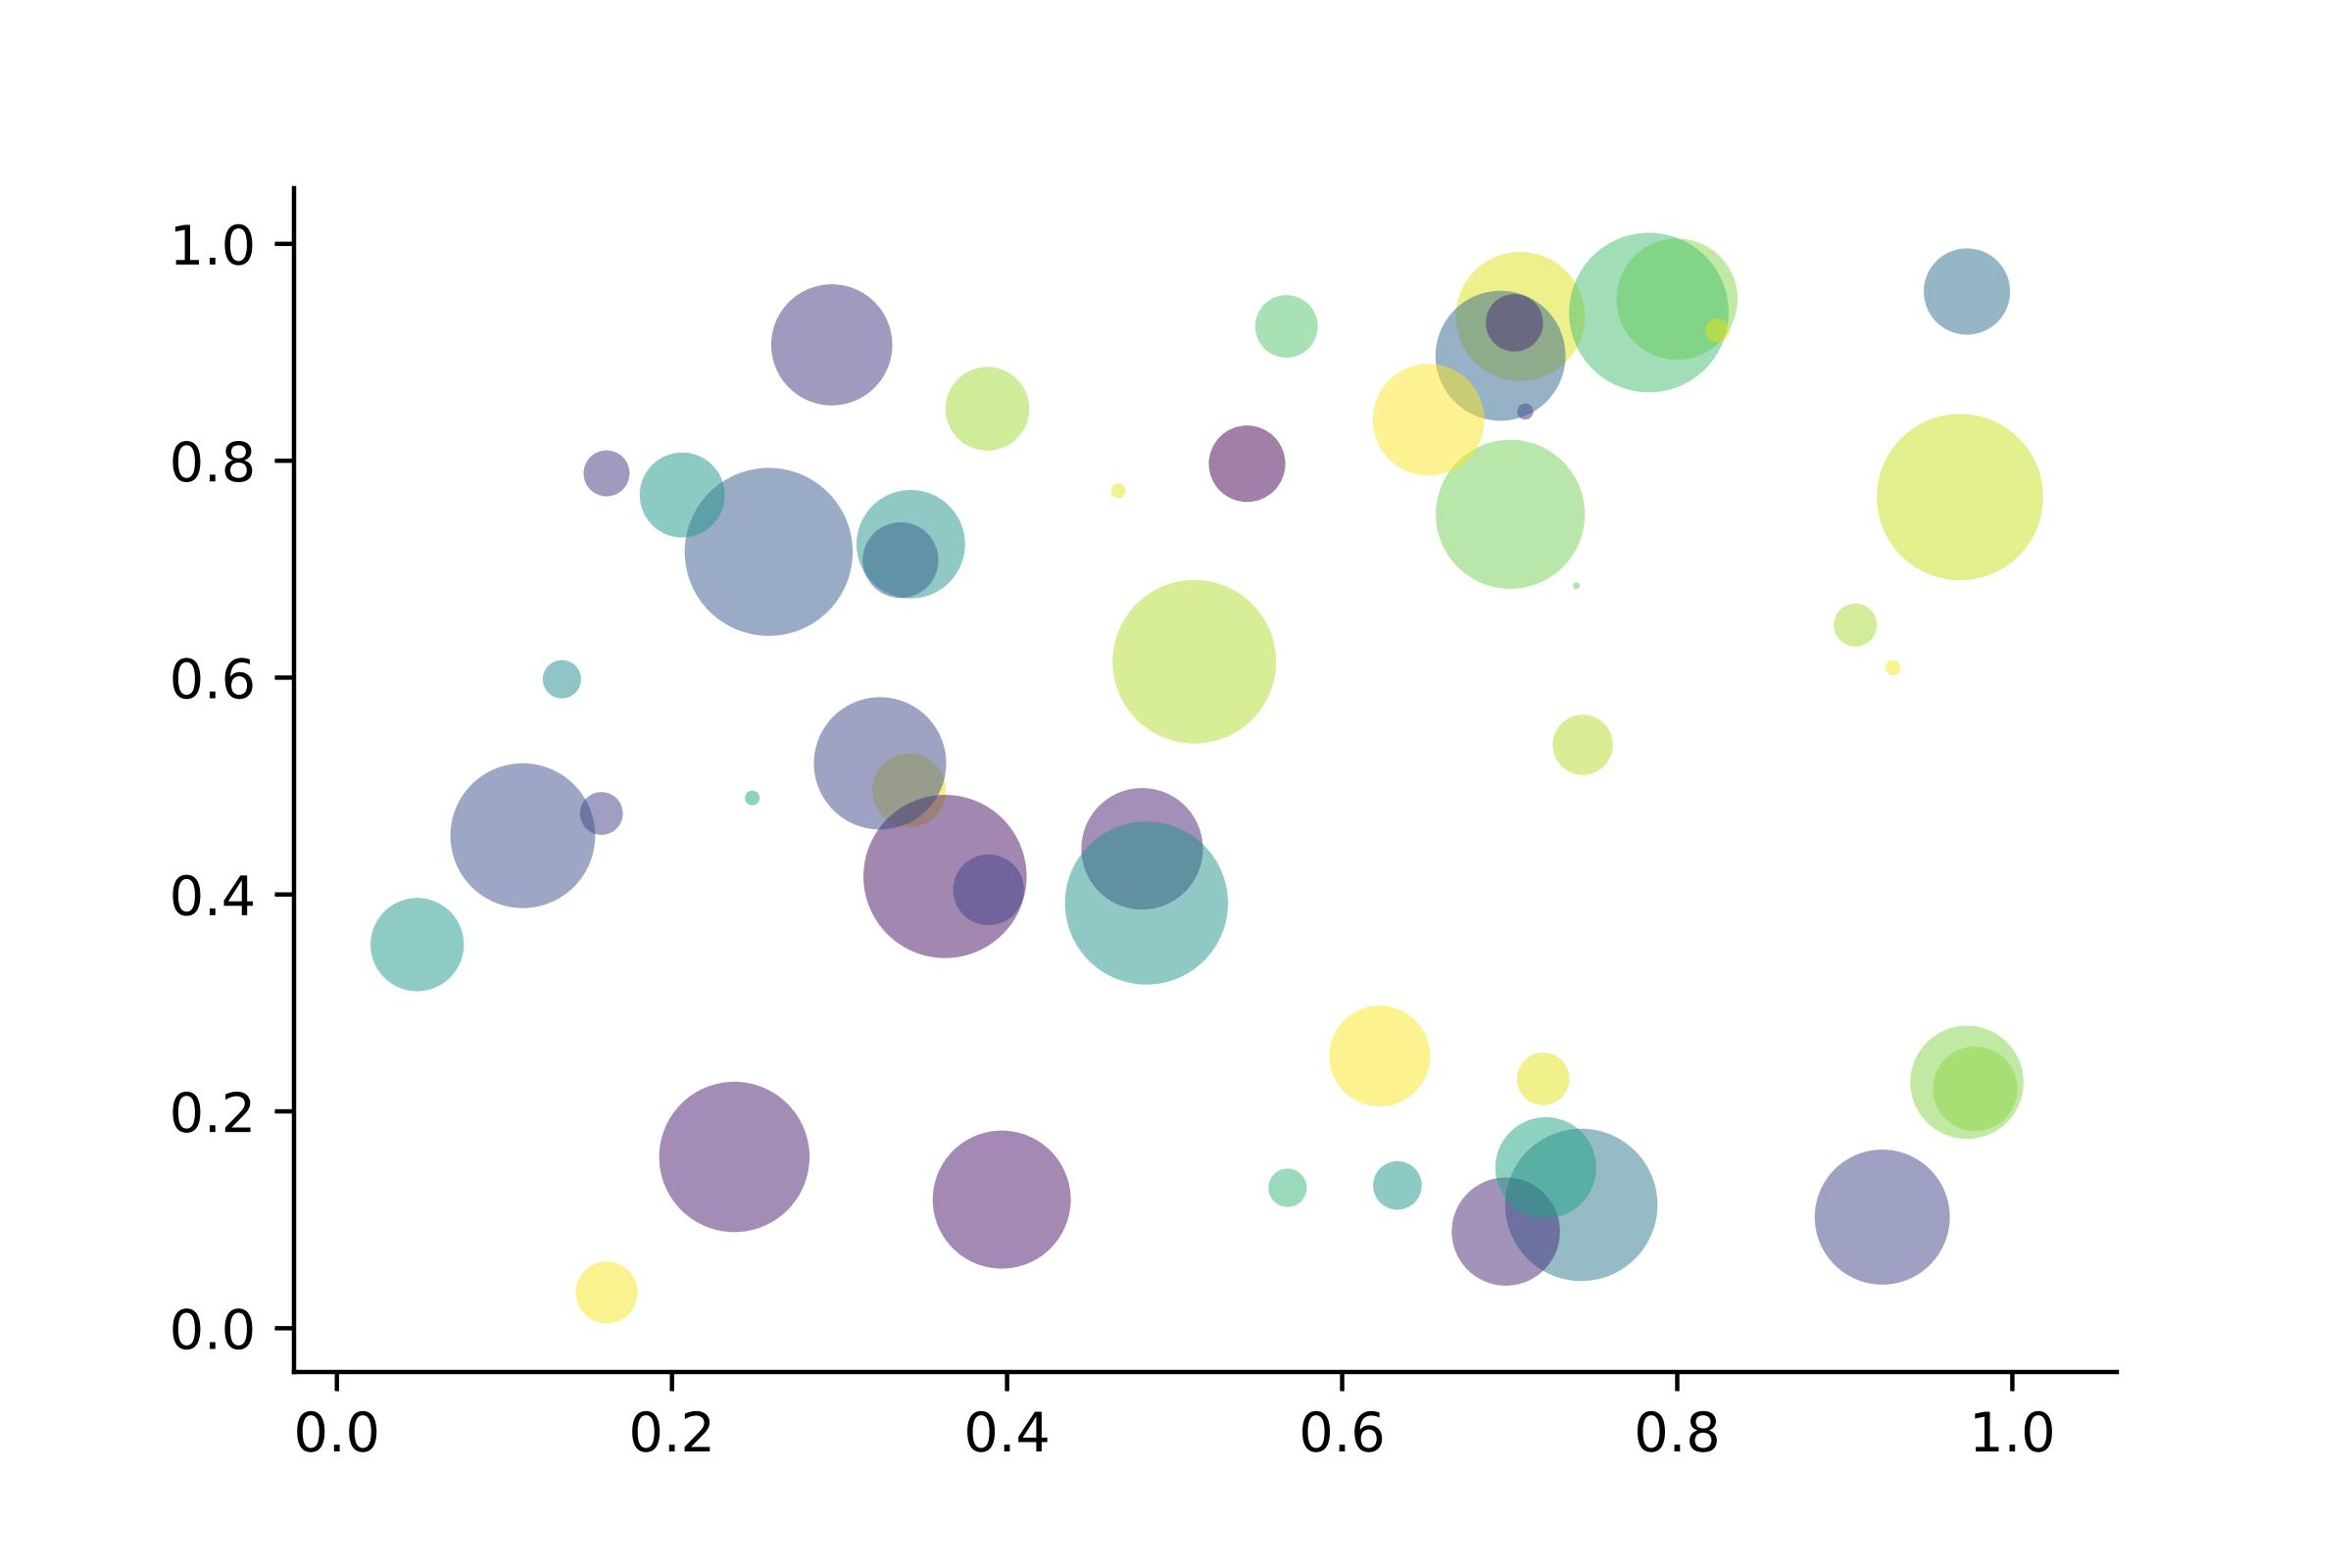
\includegraphics[width=0.4\linewidth]{image/scatter.jpg}  % 插入图片,并指定宽度为行宽的40%
    \caption{图片展示举例}  % 图片的标题或说明
    \label{fig:show}  % 为图片指定标签,方便在文档中引用
\end{figure}
 
% --------------------------------------------------------------
%     You don't have to mess with anything below this line.
% --------------------------------------------------------------

\end{document}
